\documentclass{article}
\usepackage{graphicx} %package to manage images
\usepackage[utf8]{inputenc}
\usepackage[a4paper, total={6in, 8in}]{geometry}
\usepackage{xurl}
\usepackage{hyperref}
\usepackage{float}
\title{Relatório 13 \\ ROC curves}
\author{Pedro A. S. O. Neto}
\date{Setembro, 2023}

\begin{document}

\maketitle

\section{Final ANOVAS}

Descriptive of the sample. 

\begin{table}[ht]
\centering
\begin{tabular}{rllrrr}
  \hline
 & sexo & tea & sdAgeJA & meanAgeJA & N \\ 
  \hline
1 & F & TD & 1.00 & 2.89 & 188 \\ 
  2 & F & TEA &  & 2.00 &   1 \\ 
  3 & F & nonTD & 0.83 & 3.03 &   5 \\ 
  4 & F & other & 1.59 & 2.54 &   2 \\ 
  5 & F &  & 1.06 & 3.38 &   4 \\ 
  6 & M & TD & 1.04 & 2.78 & 203 \\ 
  7 & M & TEA & 0.84 & 2.93 &  22 \\ 
  8 & M & nonTD & 0.69 & 3.48 &   8 \\ 
  9 & M & other & 0.74 & 3.15 &   4 \\ 
  10 & M &  & 0.83 & 3.05 &   7 \\ 
  11 & nan &  &  &  &   3 \\ 
   \hline
\end{tabular}
\end{table}

\begin{figure}[H]
  \caption{ANOVA alternancias}
  \noindent\makebox[\textwidth]{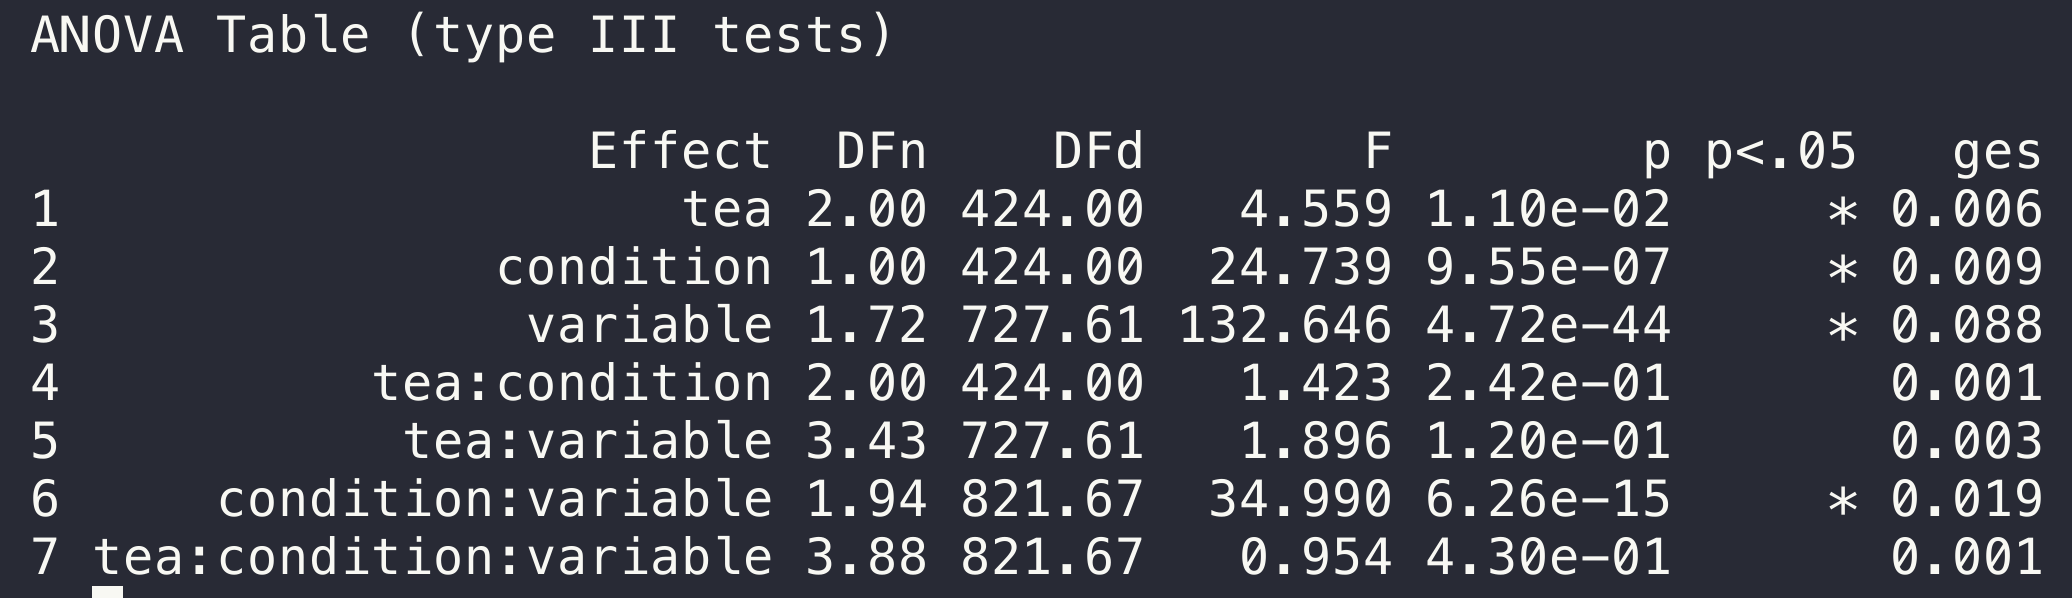
\includegraphics[scale=0.5]{./anovaAlternancia.png}}
  \centering
\end{figure}

\begin{figure}[H]
  \caption{Main effect of TEA on alternancia}
  \noindent\makebox[\textwidth]{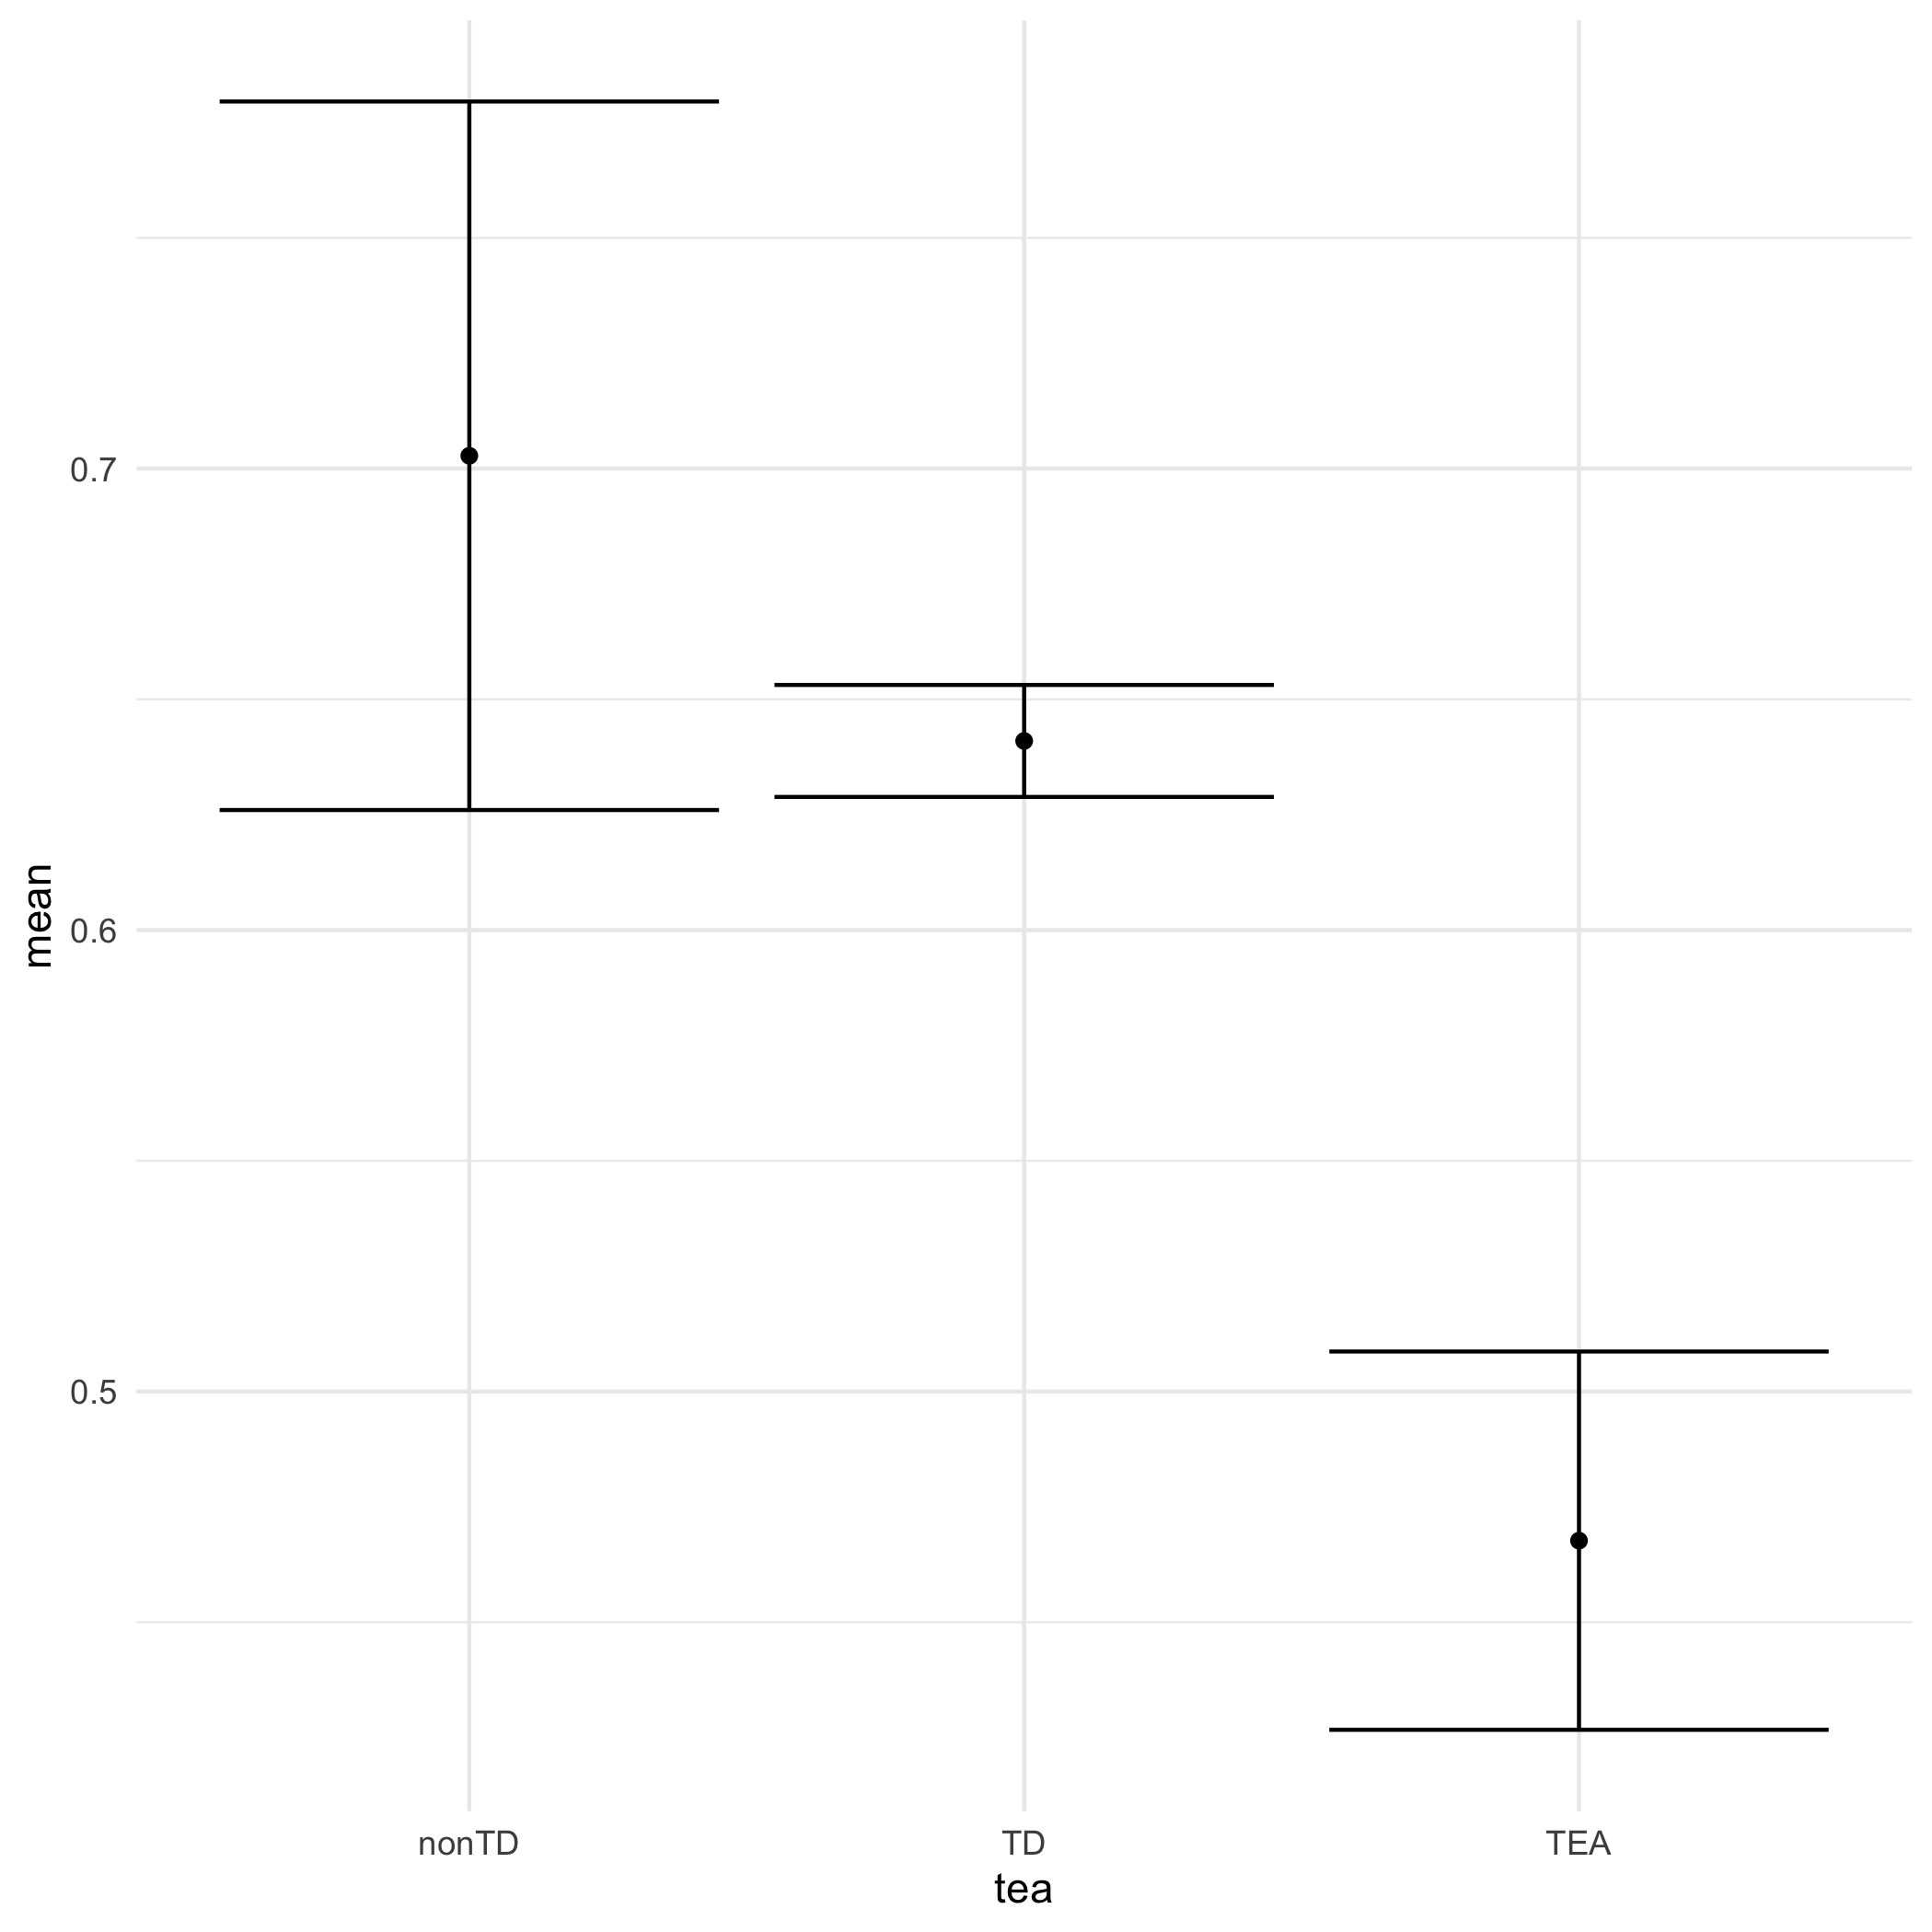
\includegraphics[scale=0.2]{./teaMainAlternancia.png}}
  \centering
\end{figure}

\begin{figure}[H]
  \caption{Main effect of variable on alternancia}
  \noindent\makebox[\textwidth]{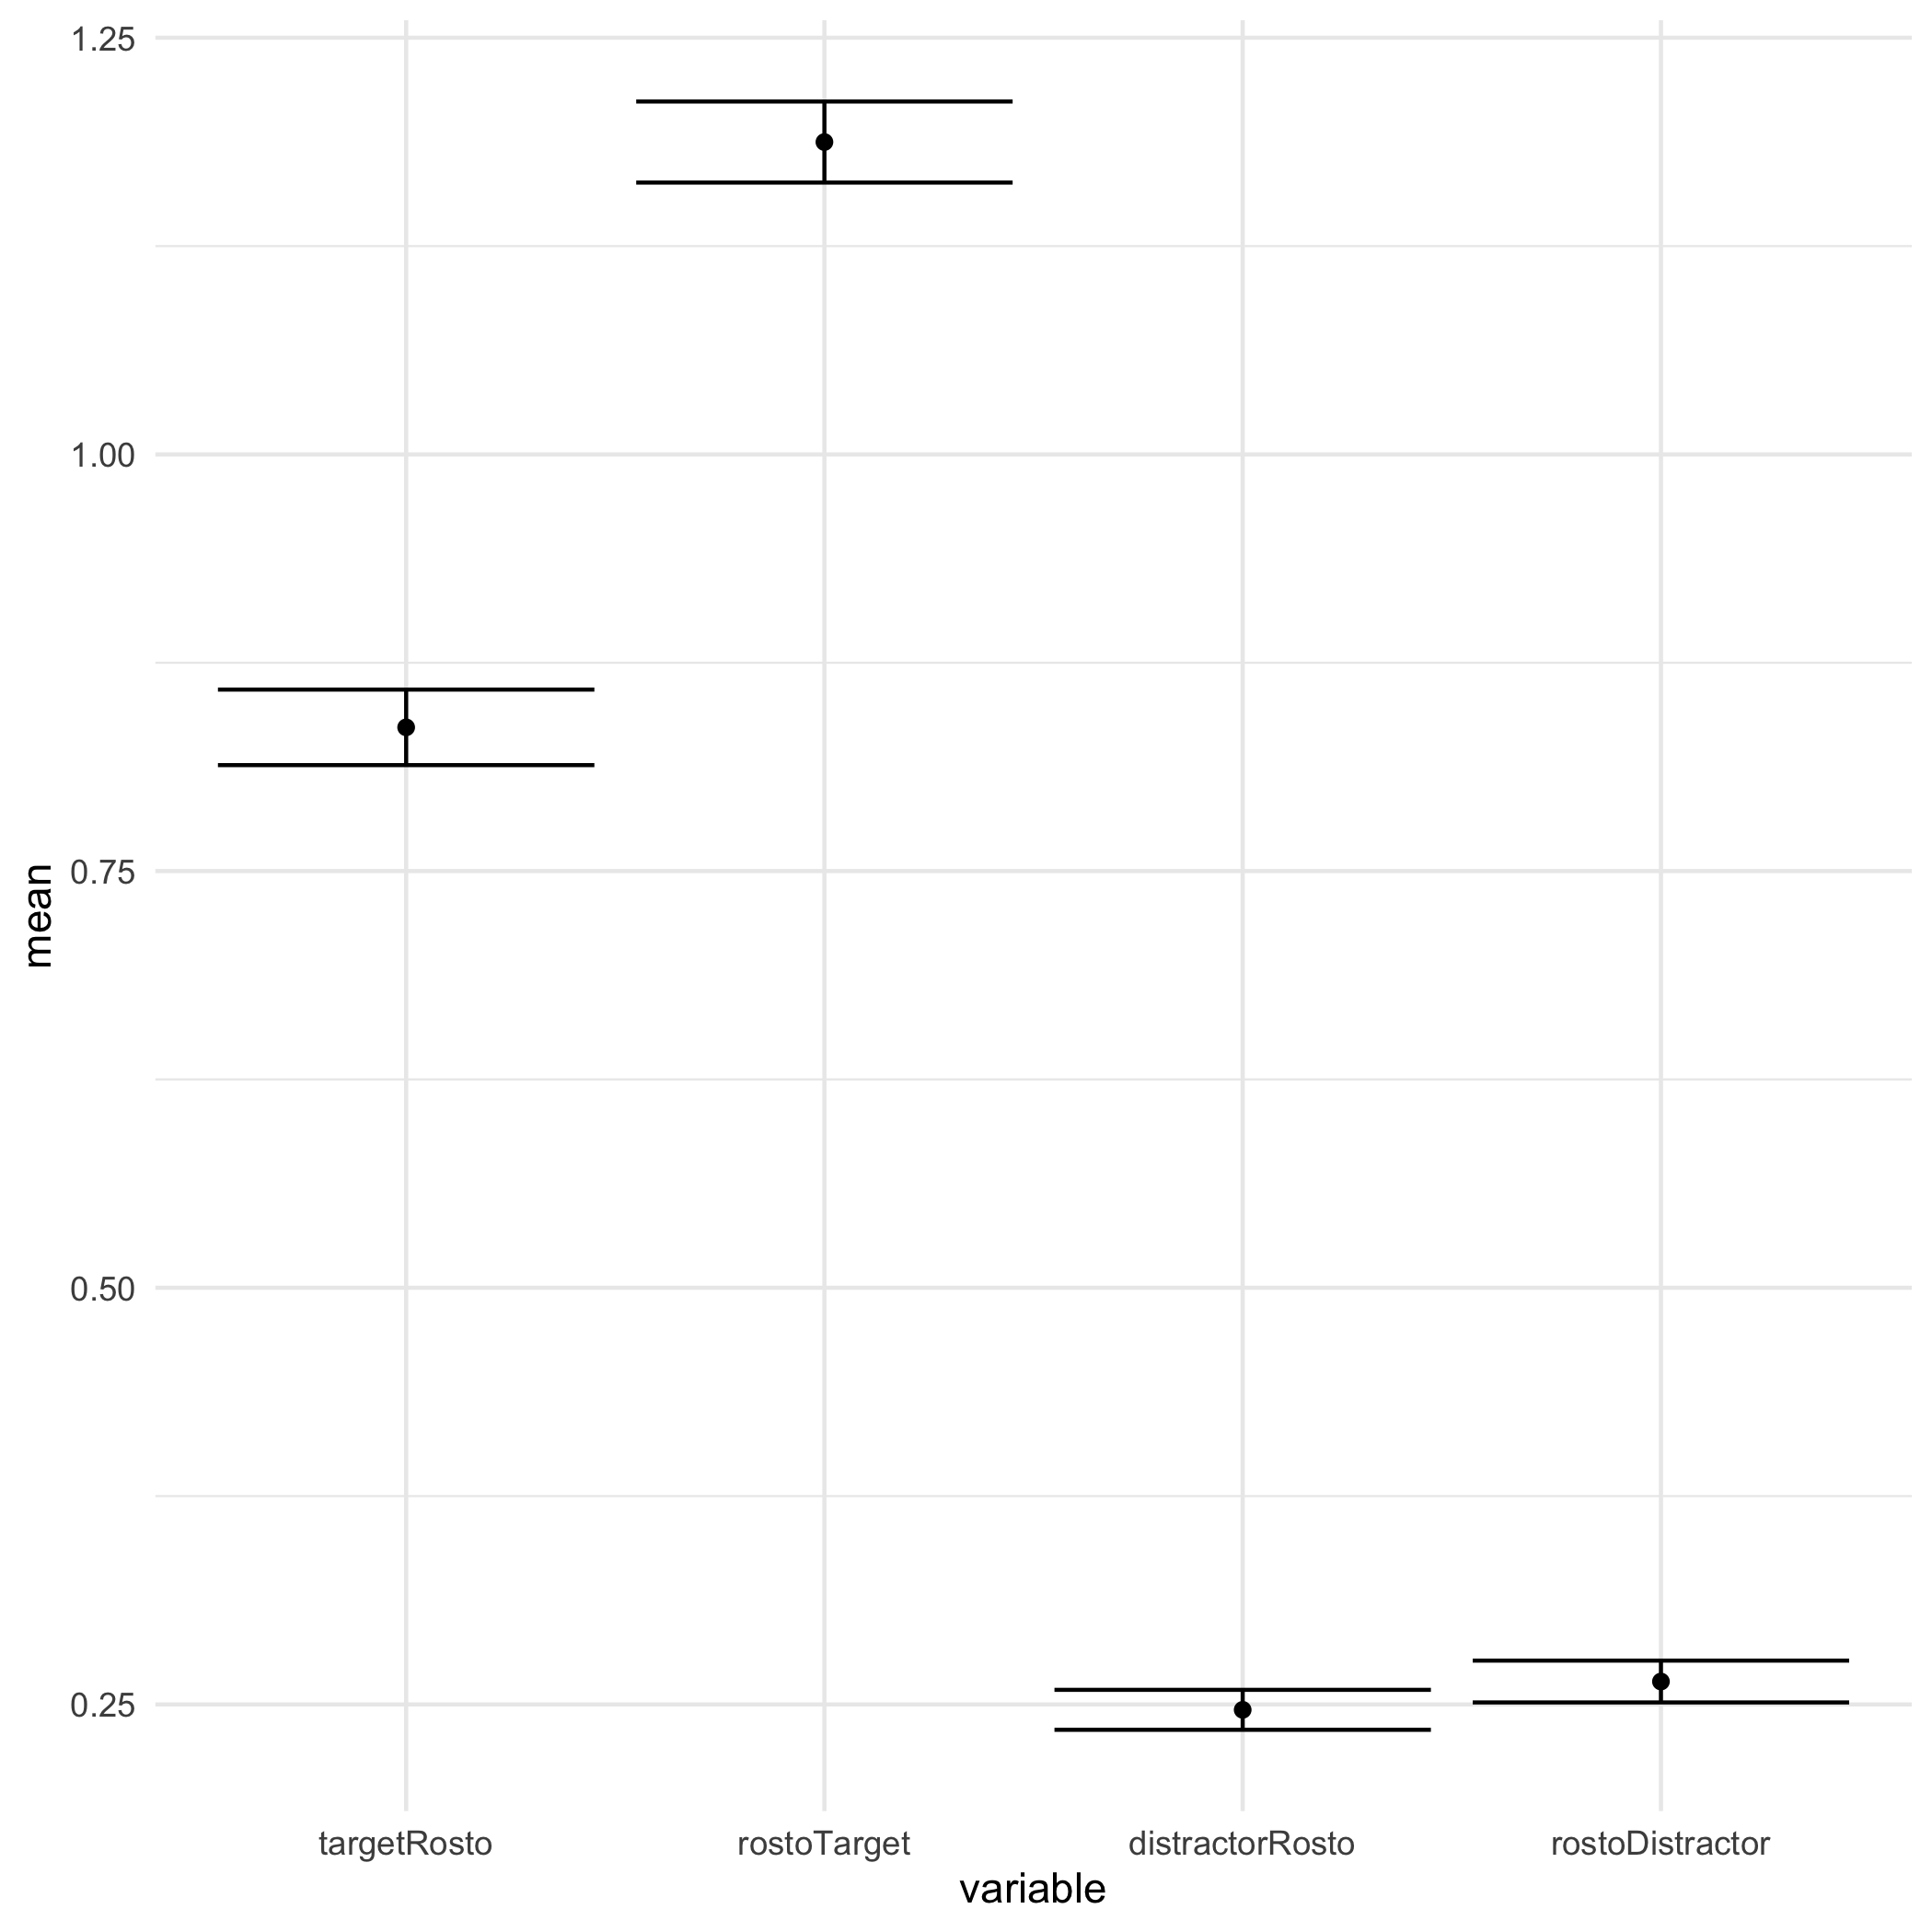
\includegraphics[scale=0.2]{./alternanciaVariable.png}}
  \centering
\end{figure}

\begin{figure}[H]
  \caption{Interaction of condition and variable on alternancia}
  \noindent\makebox[\textwidth]{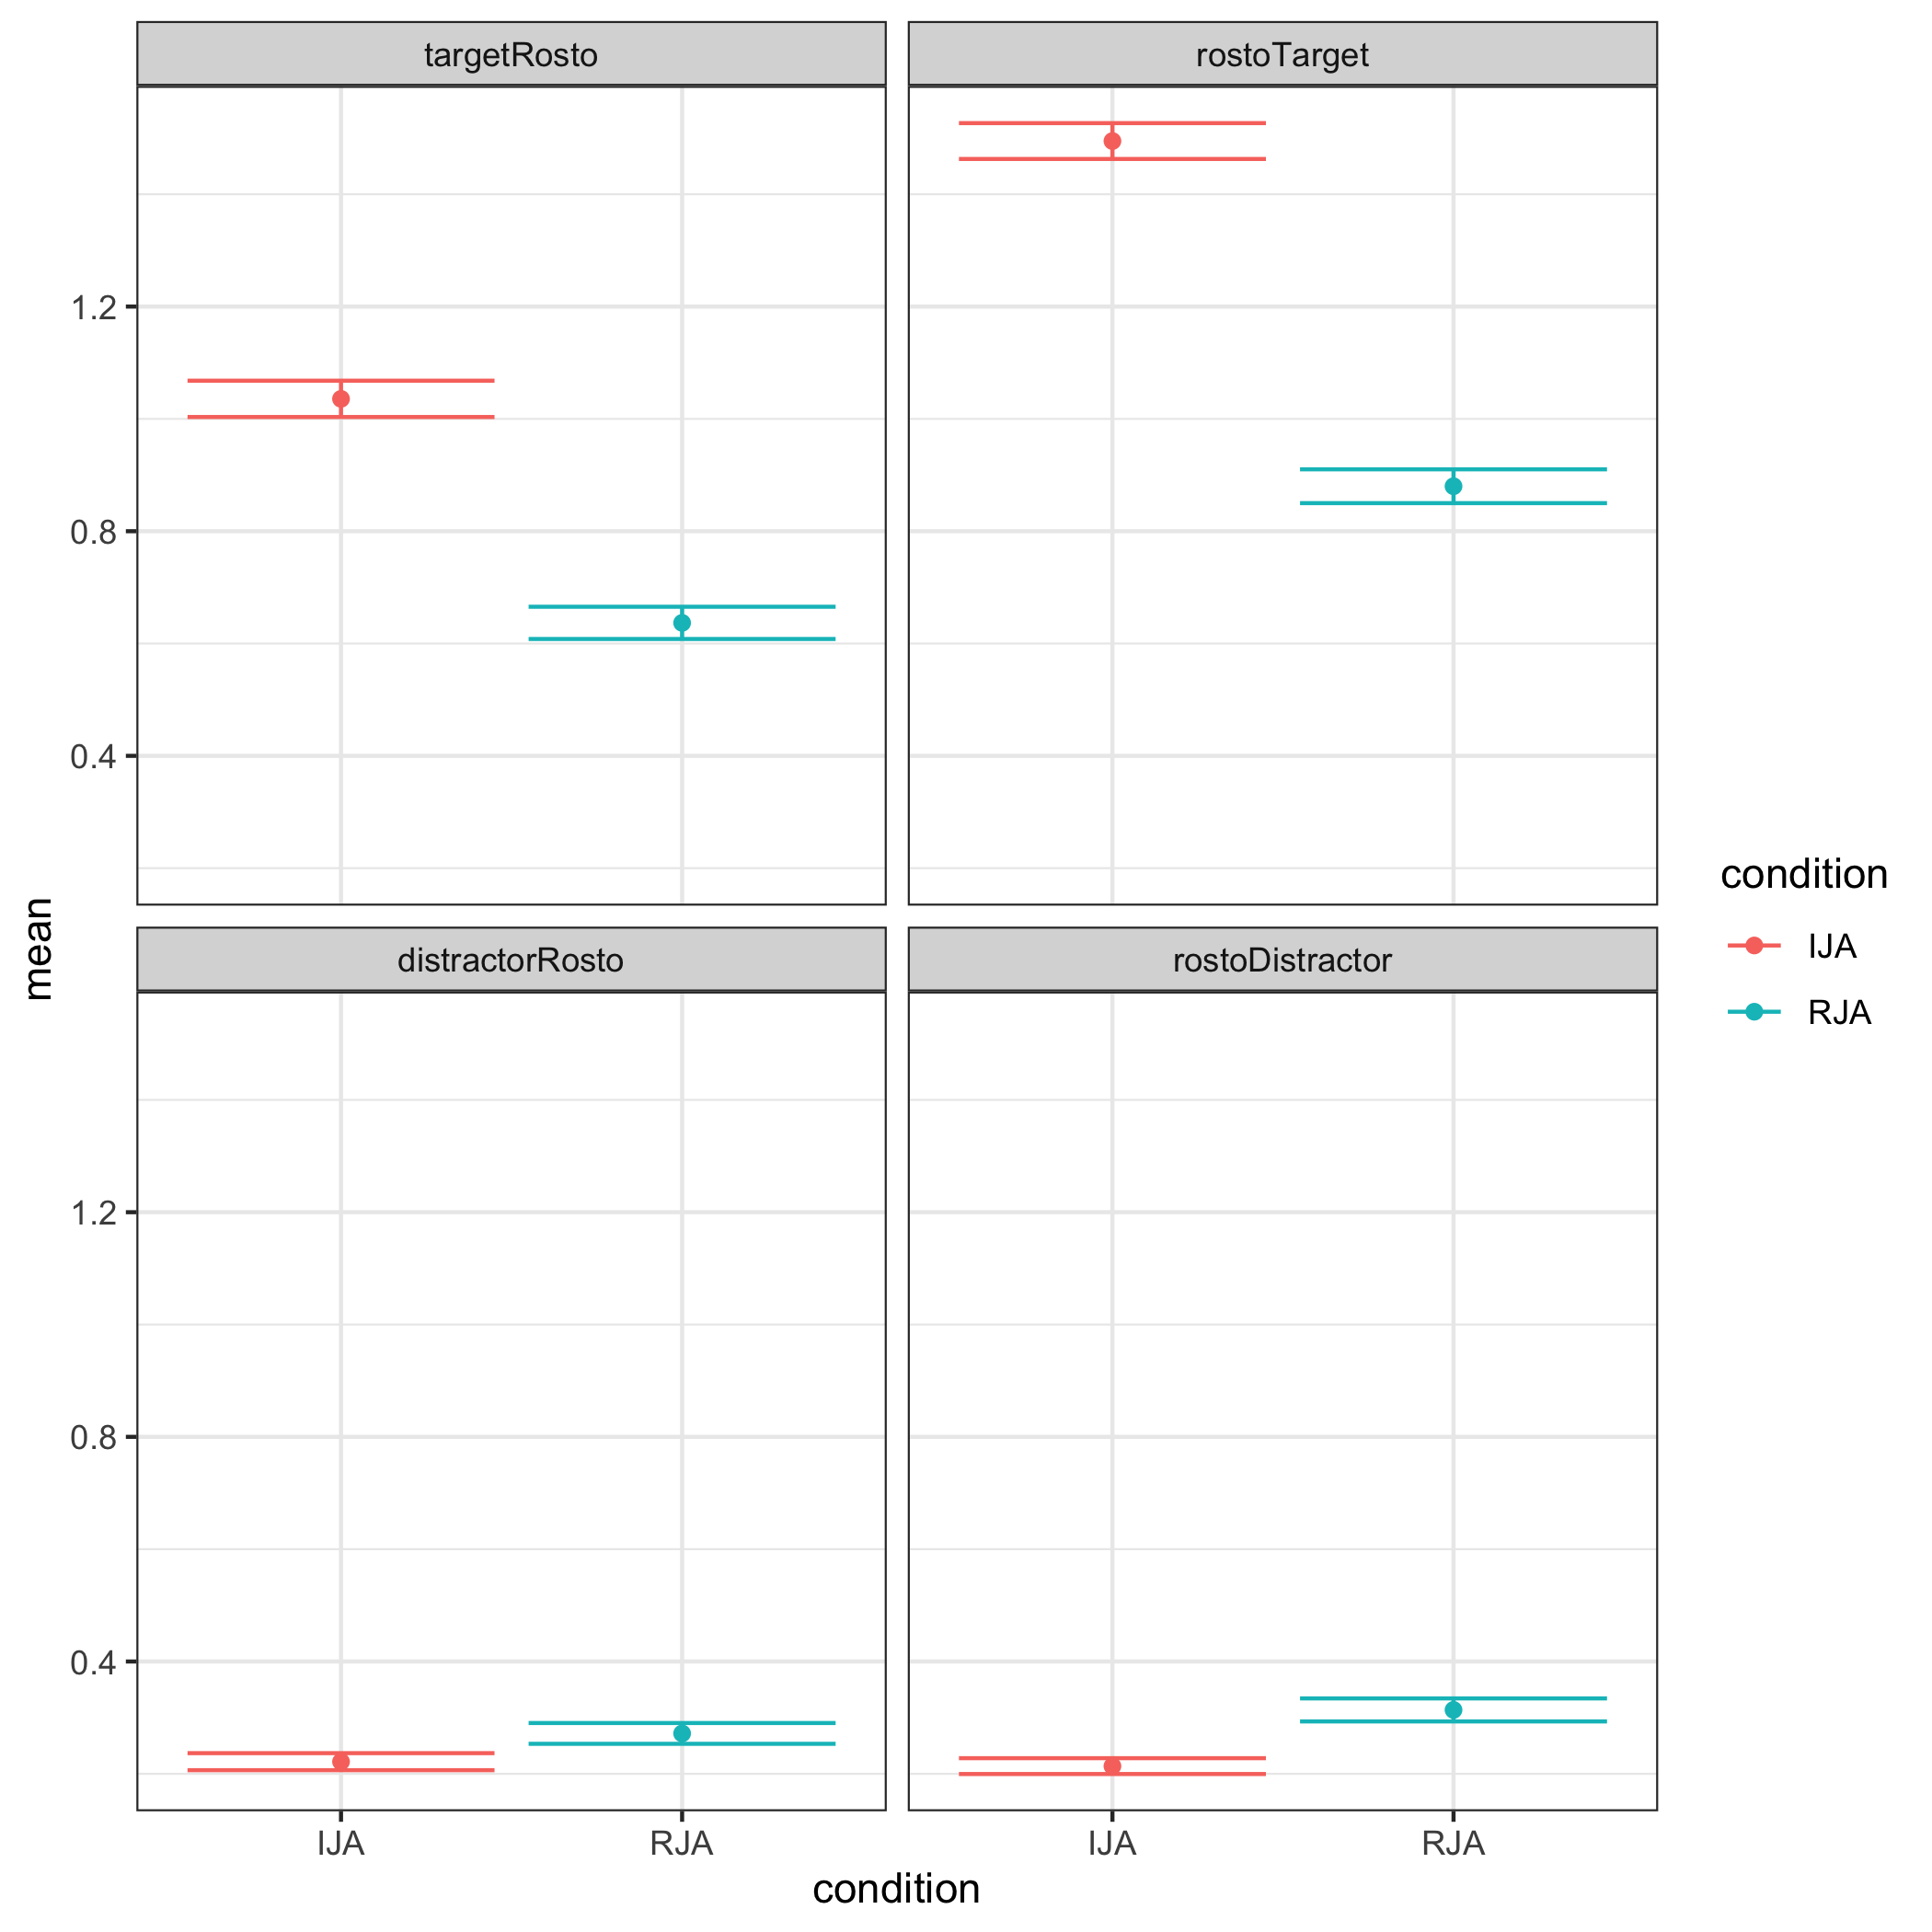
\includegraphics[scale=0.2]{./conditionVariable.png}}
  \centering
\end{figure}

\begin{figure}[H]
  \caption{Interaction of condition, variable and TEA. *not statistically significant.}
  \noindent\makebox[\textwidth]{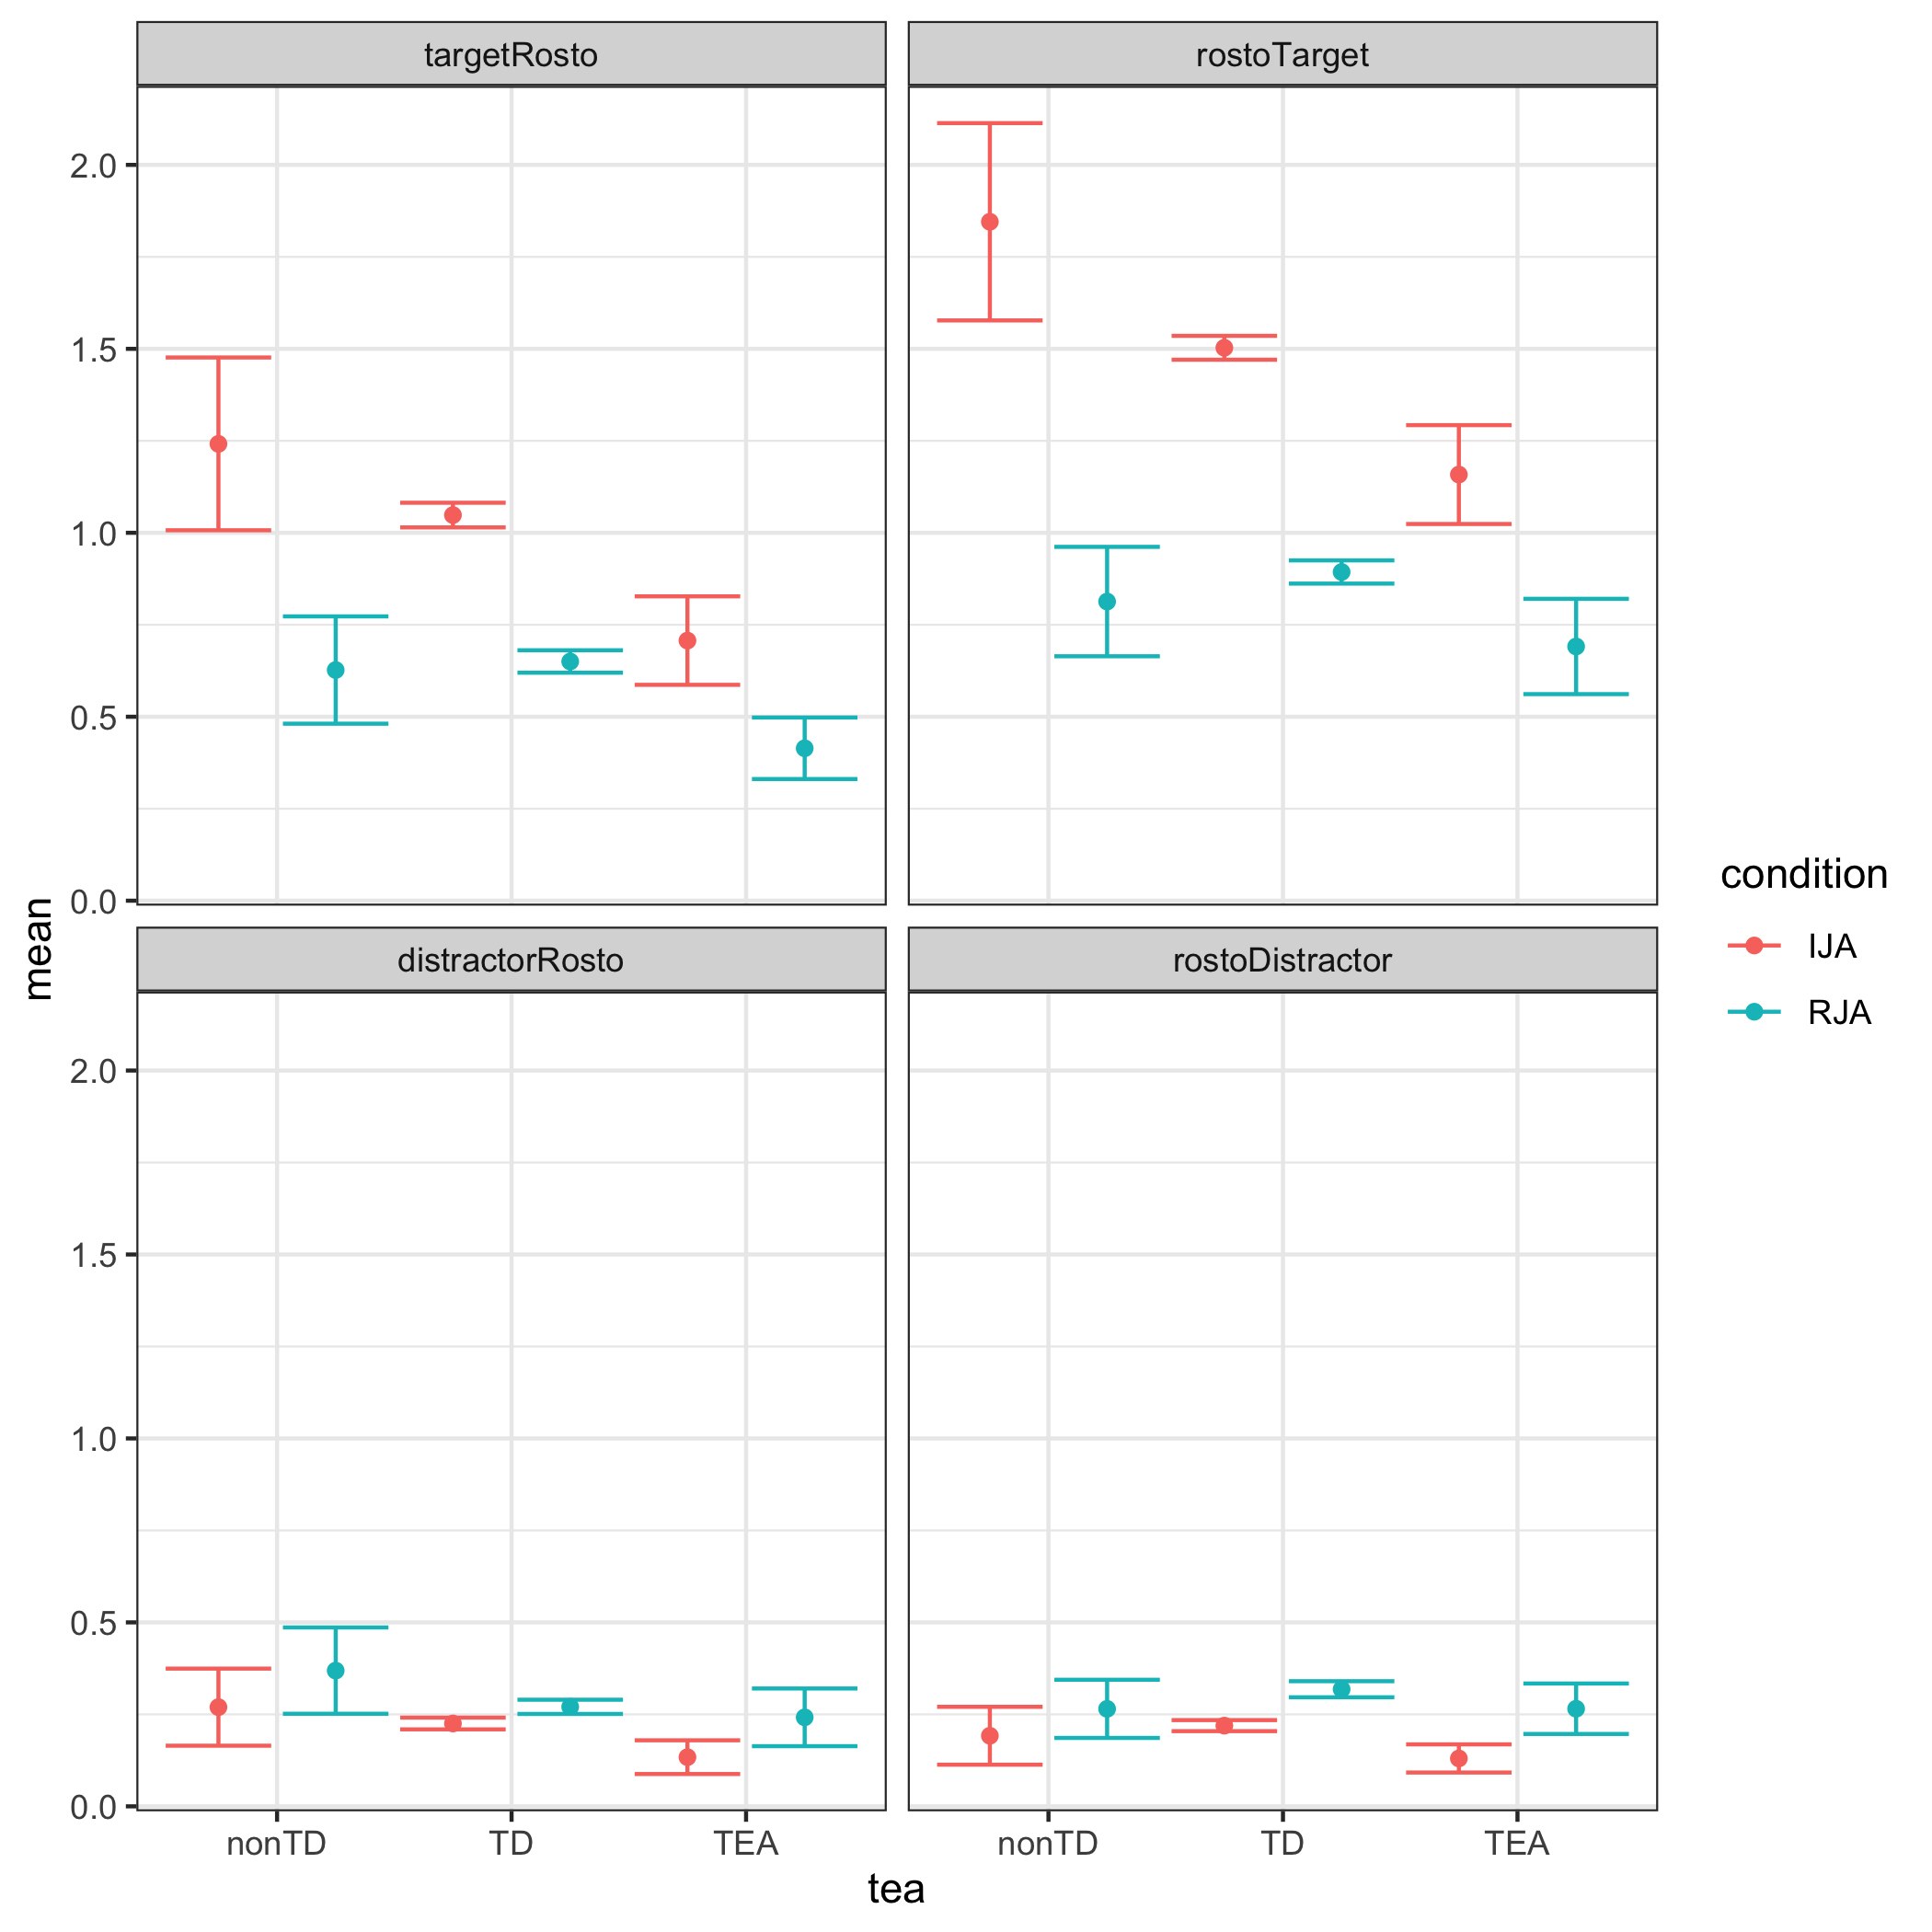
\includegraphics[scale=0.2]{./conditionVariableTea.png}}
  \centering
\end{figure}

\begin{figure}[H]
  \caption{ANOVA result for proportions}
  \noindent\makebox[\textwidth]{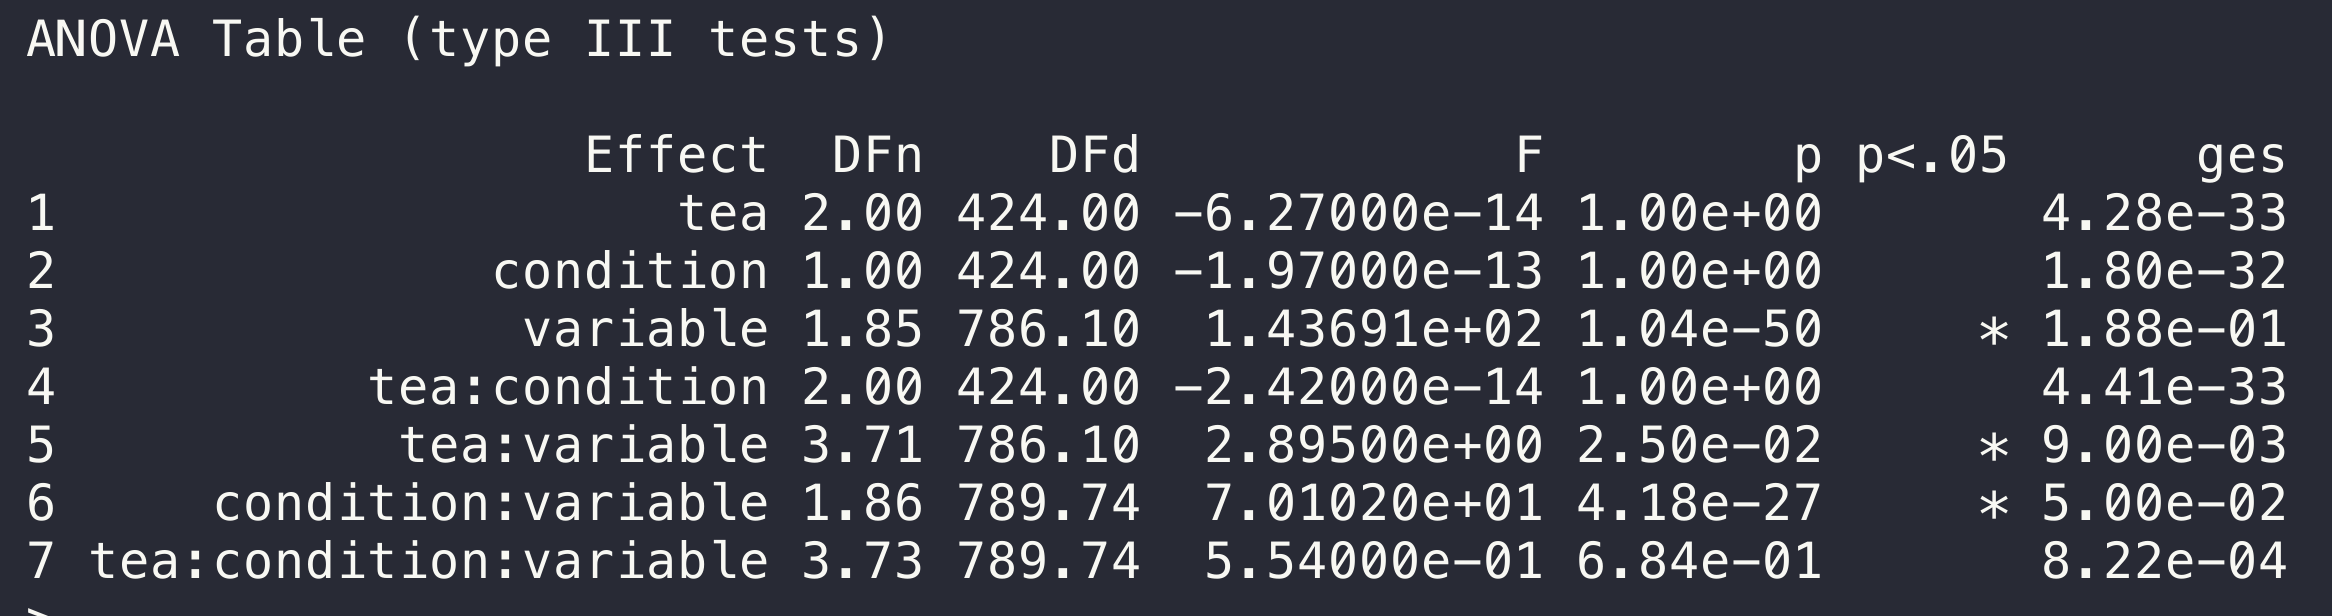
\includegraphics[scale=0.5]{./anovaProportion.png}}
  \centering
\end{figure}

\begin{figure}[H]
  \caption{Main effect of variable on proportion}
  \noindent\makebox[\textwidth]{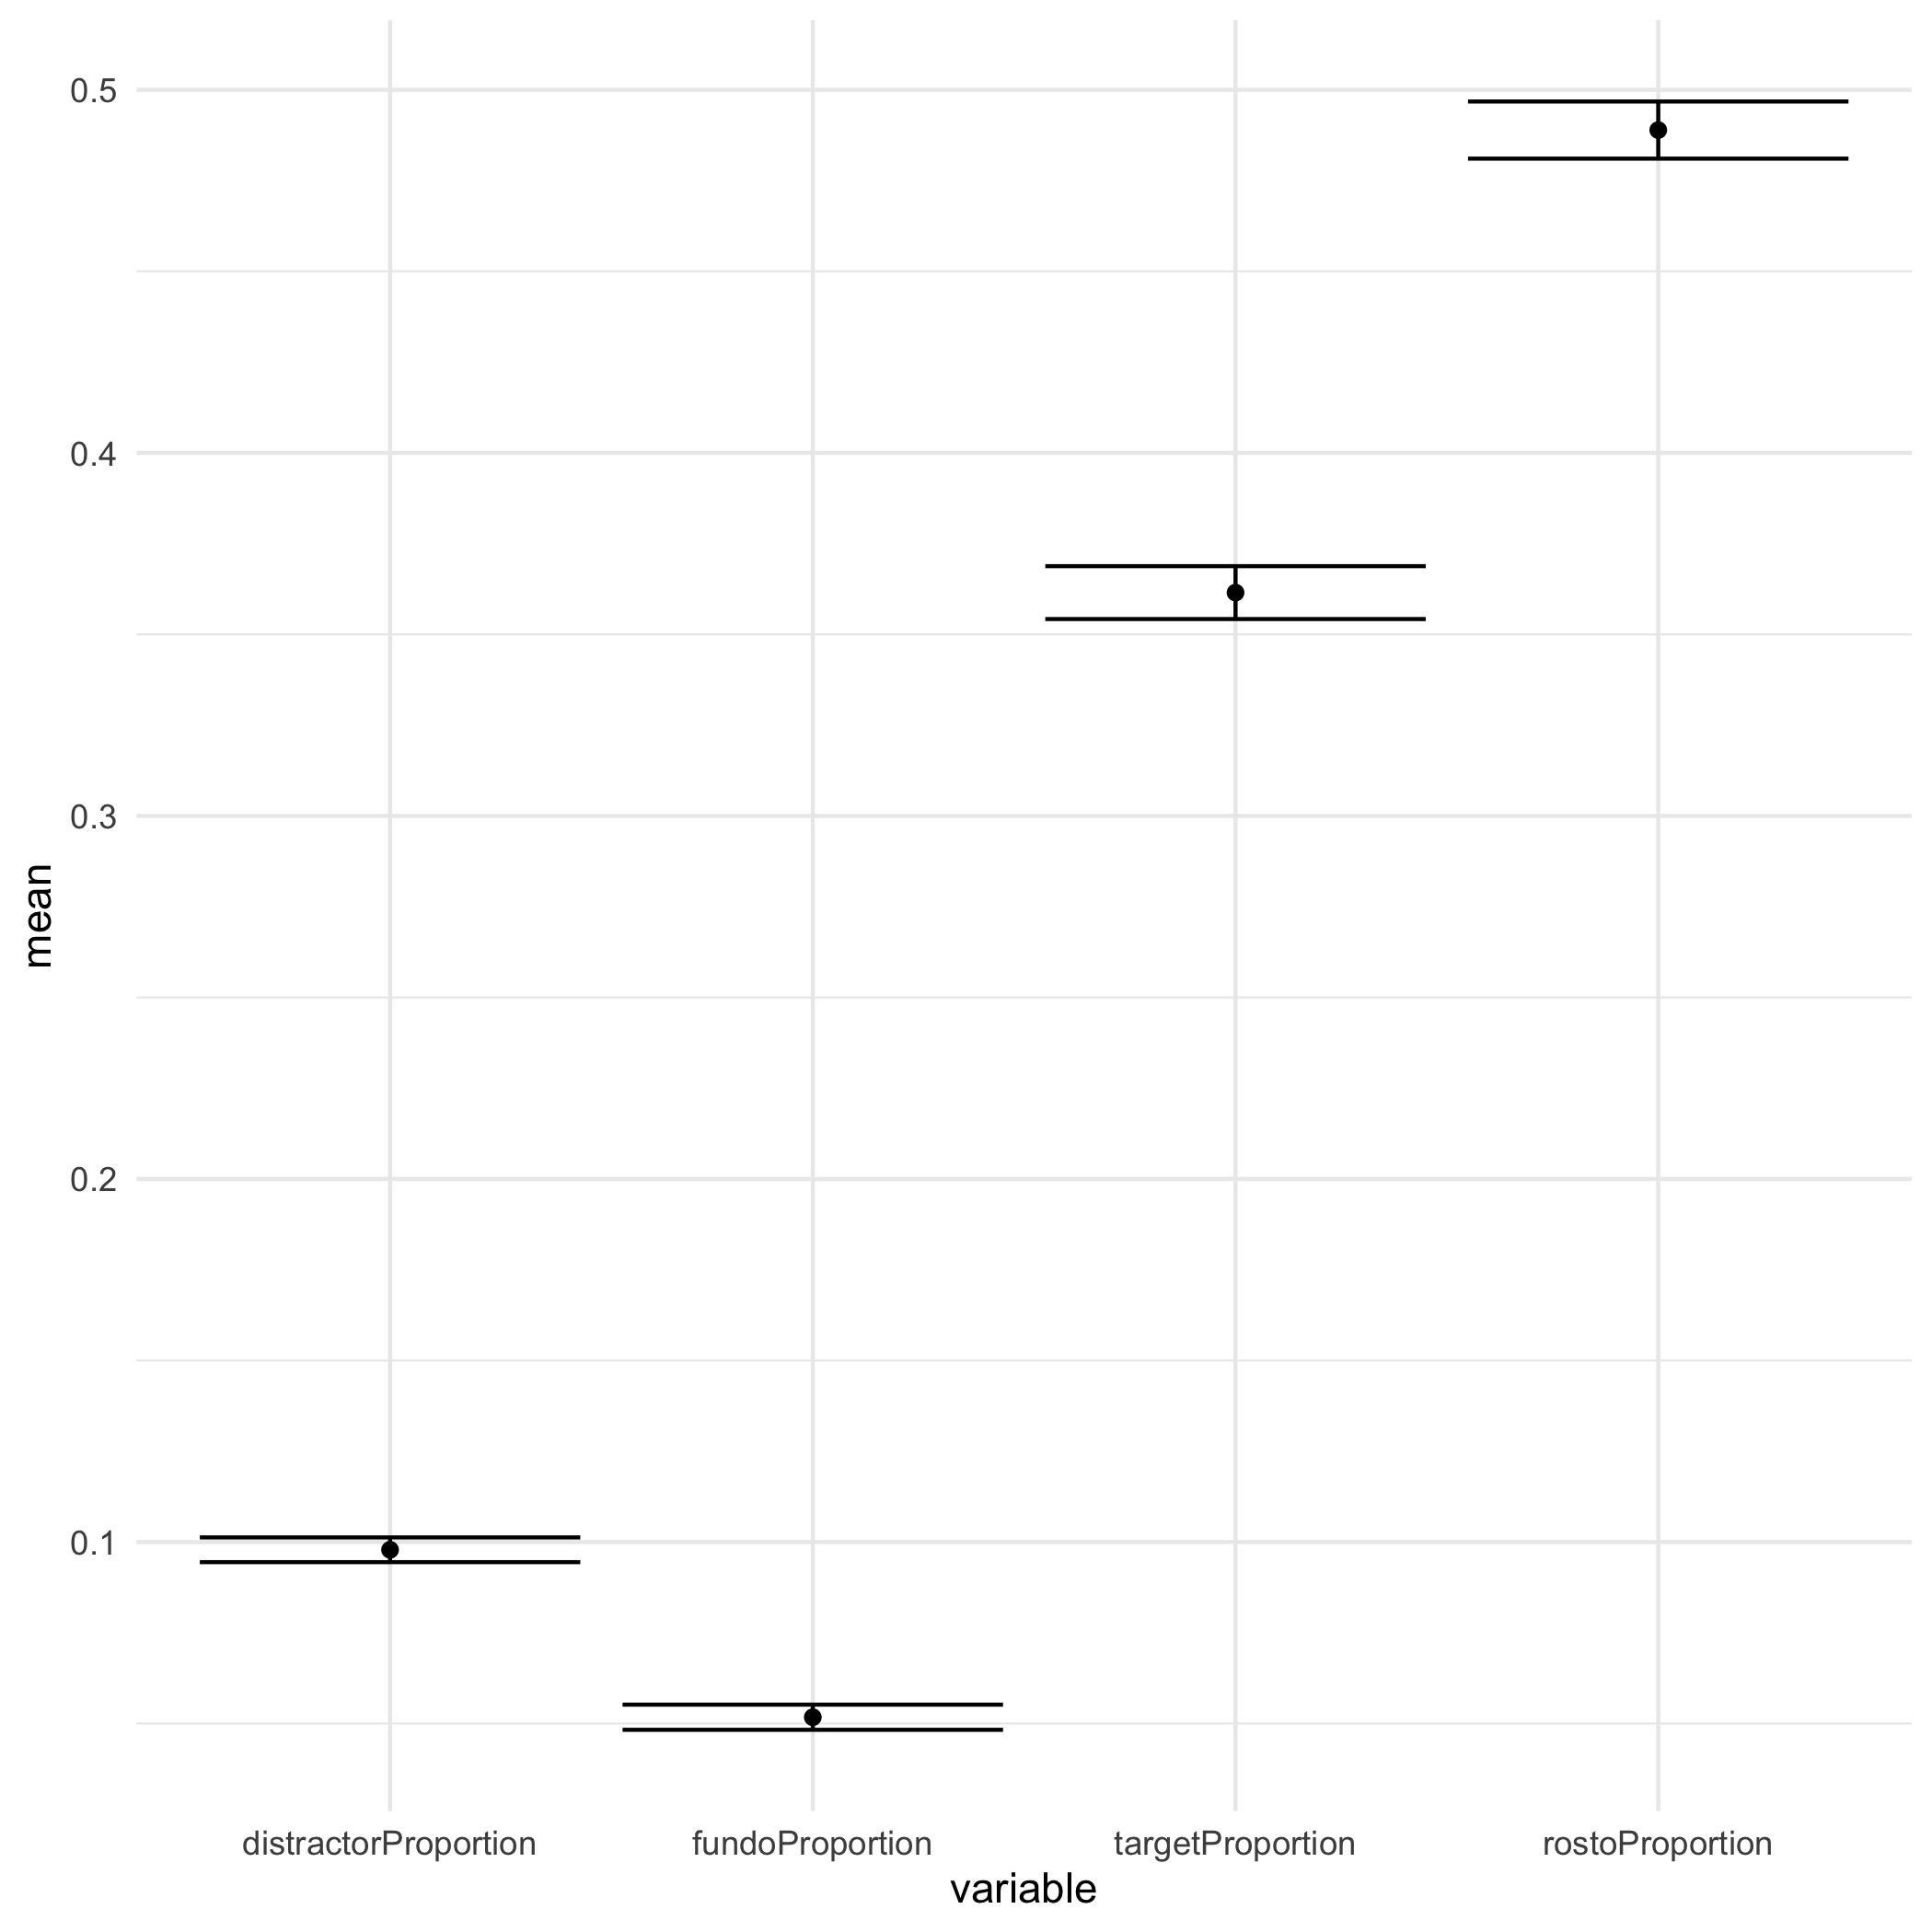
\includegraphics[scale=0.2]{./variableProportion.png}}
  \centering
\end{figure}

\begin{figure}[H]
  \caption{Interaction of tea and variable on proportion}
  \noindent\makebox[\textwidth]{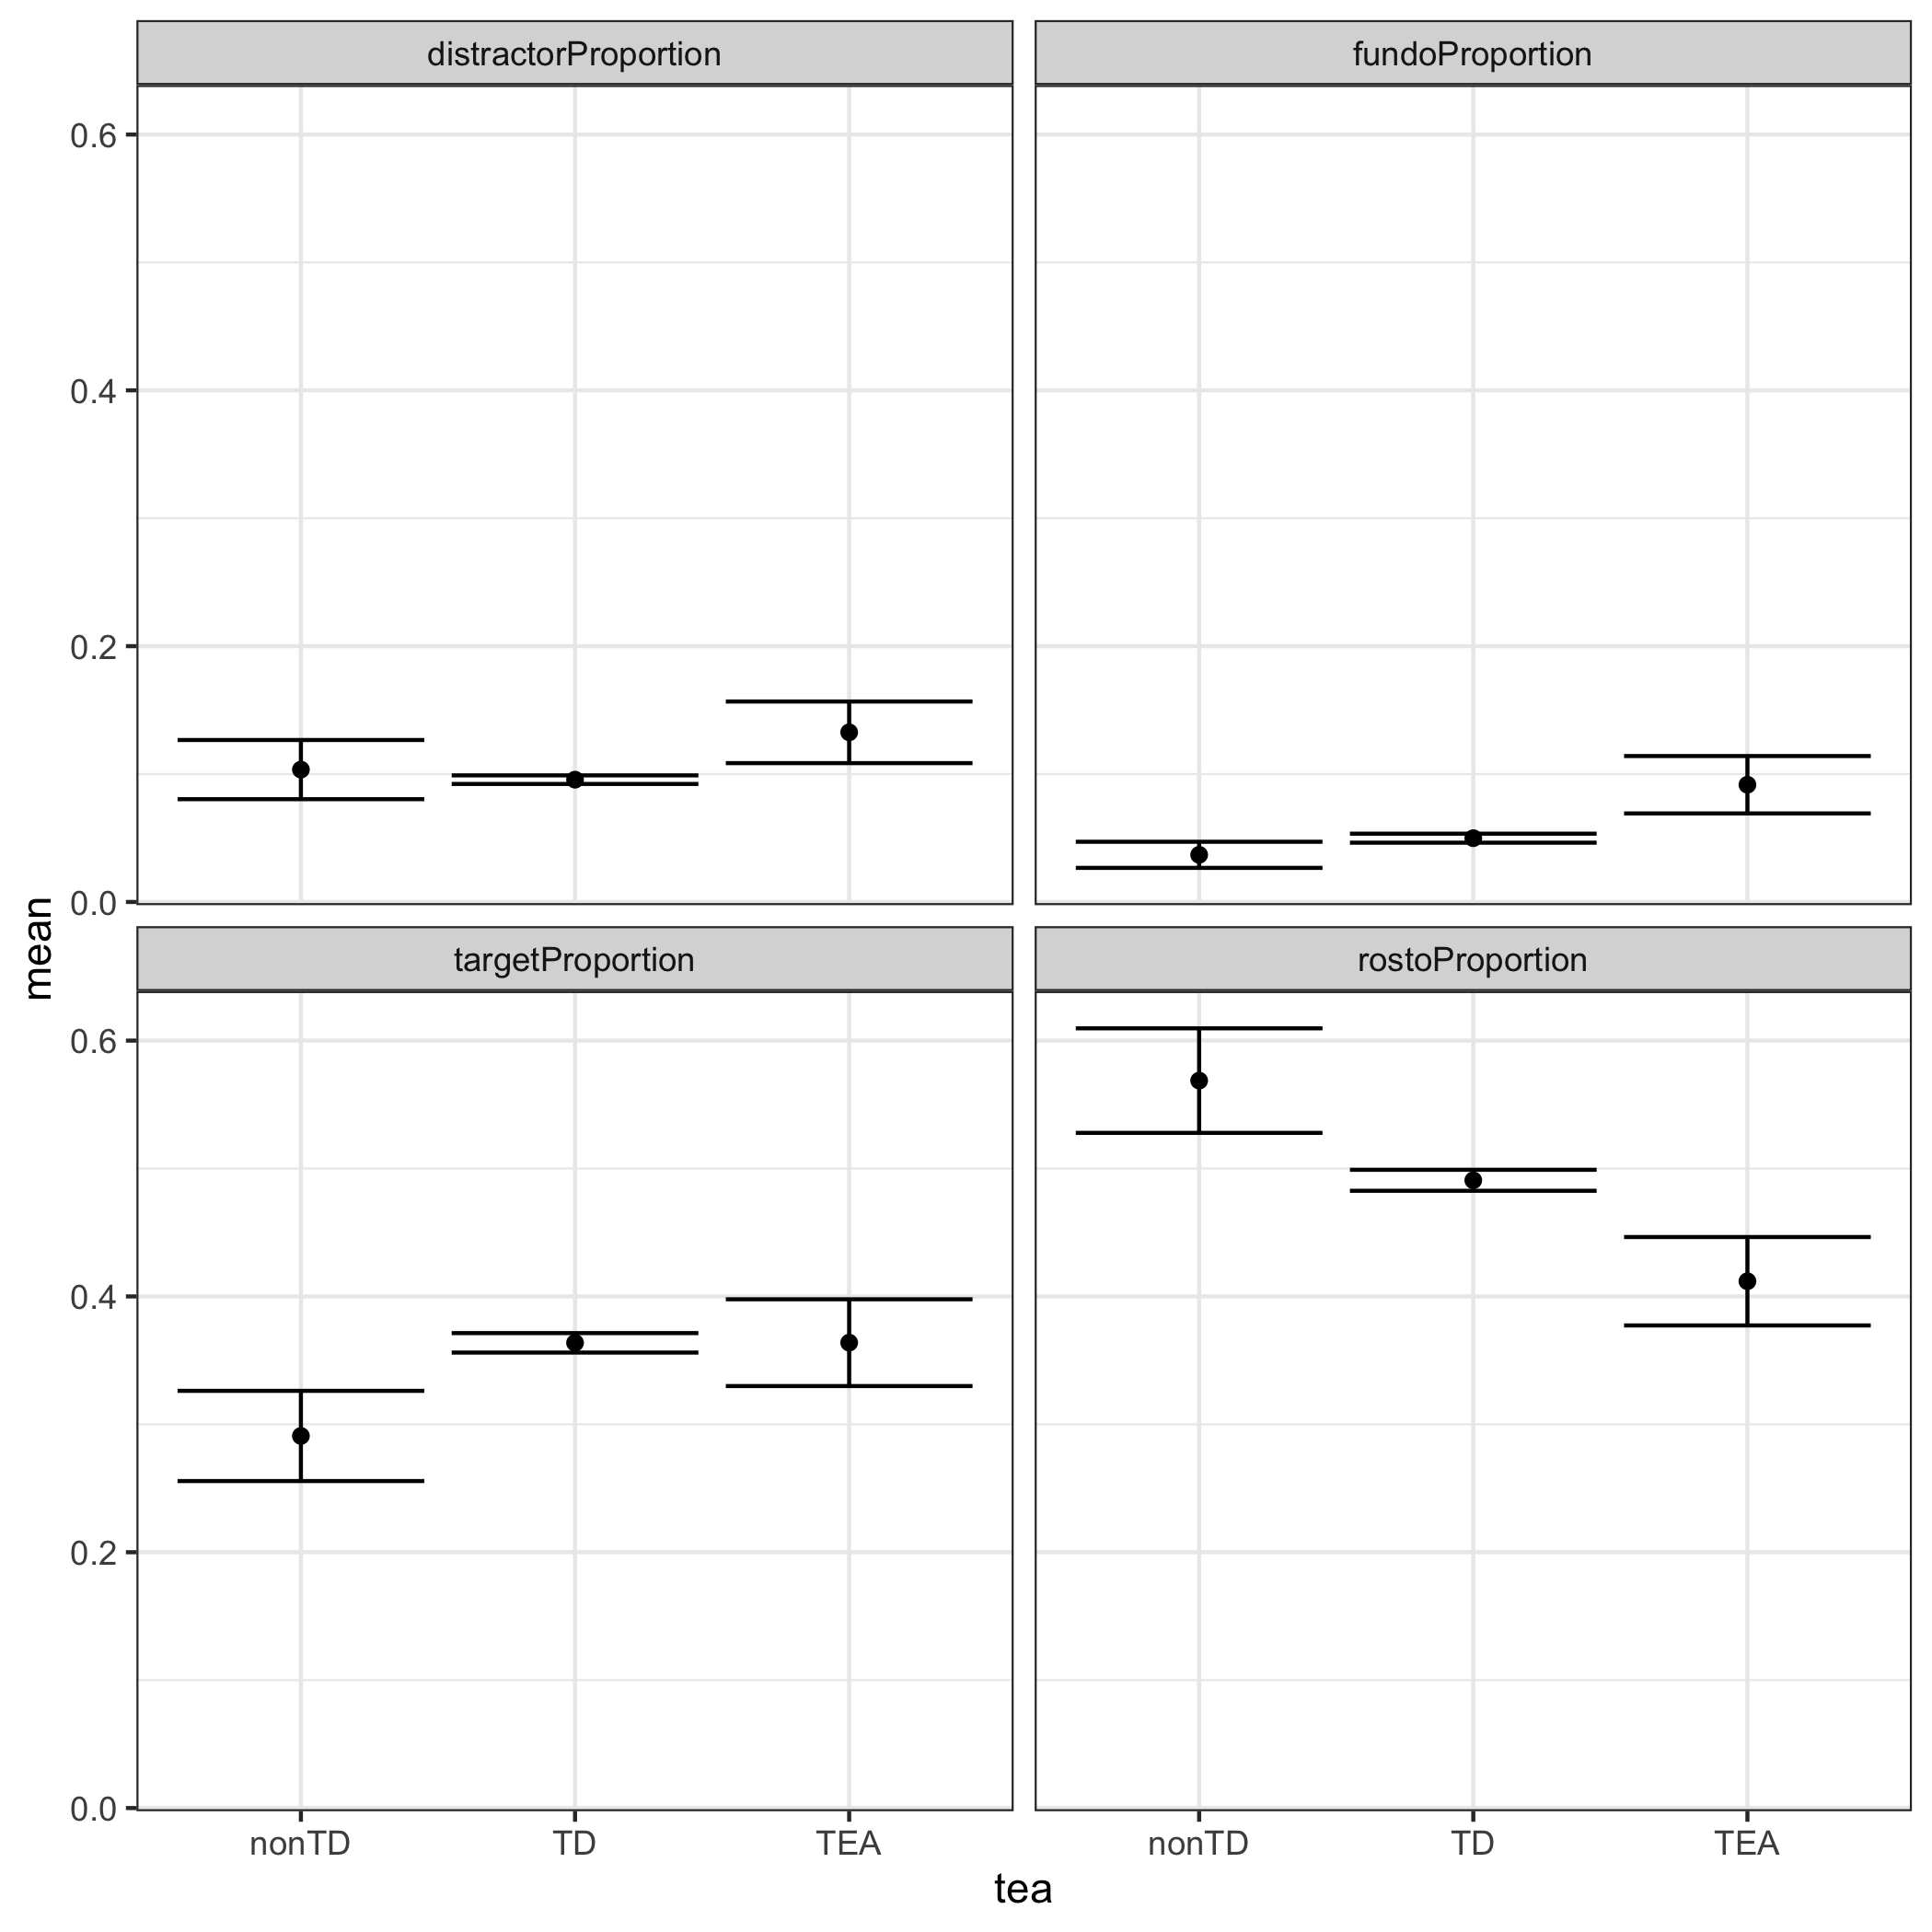
\includegraphics[scale=0.2]{./teaVariableProportion.png}}
  \centering
\end{figure}

\begin{figure}[H]
  \caption{Interaction of condition and variable on proportion}
  \noindent\makebox[\textwidth]{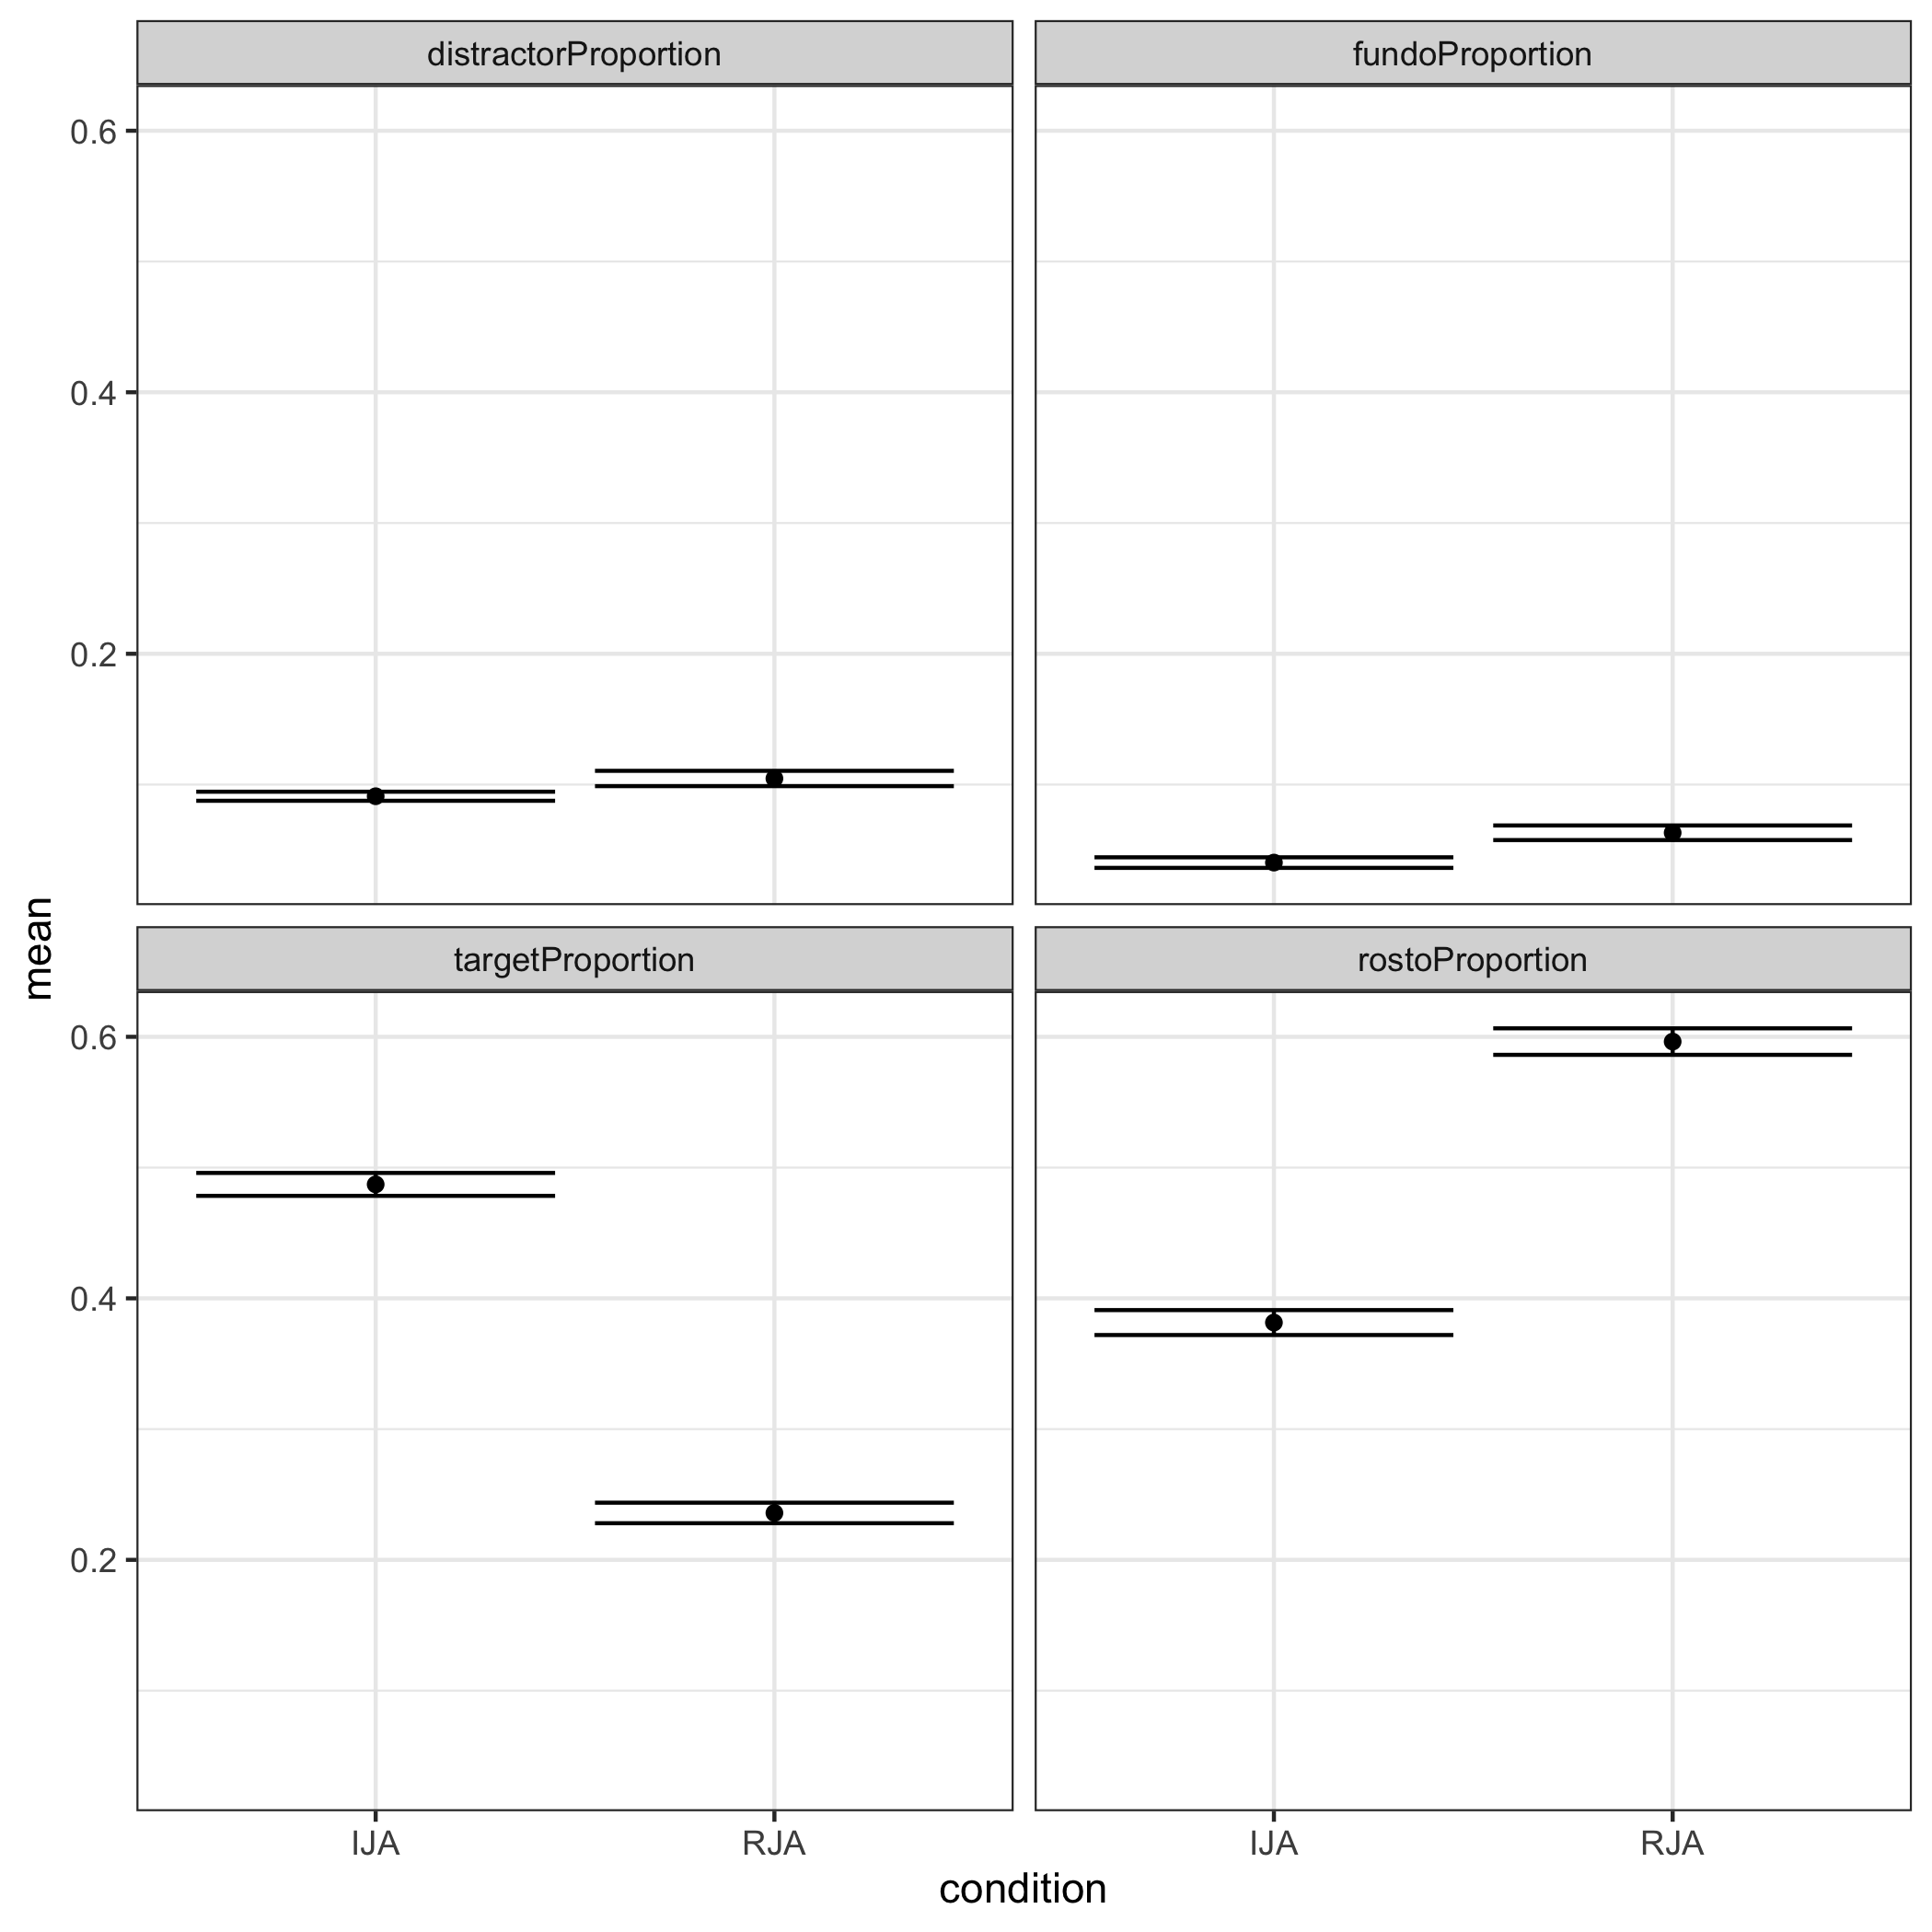
\includegraphics[scale=0.2]{./conditionVariableProportion.png}}
  \centering
\end{figure}


\end{document}
